% ============================================
%  Article Class (This is a LaTeX2e document)  
% ============================================
\documentclass[12pt]{scrartcl}

\usepackage[english]{babel}
\usepackage[utf8]{inputenc}

\usepackage{enumitem}
\usepackage[round]{natbib}
\usepackage{color}

\newcommand\reft[3][]{#2~\ref{#3}#1}
\newcommand\refp[3][]{(#2~\ref{#3}#1)}
\newcommand\refsect[1]{\reft{Section}{#1}}
\newcommand\refsecp[1]{\refp{Sec.}{#1}}
\newcommand\reftabt[1]{\reft{Table}{#1}}
\newcommand\reftabp[1]{\refp{Tab.}{#1}}

% ======
%  Math
% ======
\usepackage{amsmath}
\usepackage{amsthm}
\usepackage{mathtools} % \mathclap
\newtheorem{thm}{Theorem}[section]
\newtheorem{cor}[thm]{Corollary}
\newtheorem{lem}[thm]{Lemma}
\newtheorem{prop}[thm]{Proposition}
\newtheorem{property}[thm]{Property}
\theoremstyle{definition}
\newtheorem{defn}[thm]{Definition}
\newtheorem{assum}[thm]{Assumption}
\theoremstyle{remark}
\newtheorem{rem}[thm]{Remarque}
\numberwithin{equation}{section}
\newtheorem{req}[thm]{Requirement}

\usepackage{amssymb}
\newcommand{\prob}[1]{\mathbb{P}\left(#1\right)}
\newcommand{\Ker}[1]{\mathrm{Ker}\left(#1\right)}
\newcommand{\Image}[1]{\mathrm{Im}\left(#1\right)}
\newcommand{\diag}[1]{\mathrm{diag}\left(#1\right)}
\newcommand{\Vect}[1]{\mathrm{Vect}\left\{#1\right\}}

% ============================
%  Figures and relative paths
% ============================
\usepackage{graphicx}
\graphicspath{{figures/}}
\usepackage{import}
\makeatletter
  \def\relativepath{\import@path}
\makeatother
\newcommand\reffigt[2][]{\reft[#1]{Figure}{#2}}
\newcommand\reffigp[2][]{\refp[#1]{Fig.}{#2}}

% ==========
%  Document
% ==========
\begin{document}

\title{RBA pipeline}%
\author{S. Fischer - Biosys - MAIAGE}%
\date{\today}%

\maketitle

\newpage

\tableofcontents

\newpage

\section{Description of workflow}

\reffigt{fig:workflow} shows the global workflow of the pipeline. It contains three parts:
\begin{enumerate}
\item \textbf{preRBA}: Parsing of biological data into RBA compatible XML files. Parts of the process are semi-automated, meaning the user is needed to help solve ambiguous annotations.
\item \textbf{buildRBA}: XML files are transformed into matrices used by the RBA solver and stored into optimized matlab structures.
\item \textbf{solveRBA}: matrices are used to compute the optimal resource allocation.
\end{enumerate}
As a first step, this workflow should run for any prokaryote.

\begin{figure}[ht]
  \centering
  \includegraphics[width=\linewidth]{workflow}
  \caption{Workflow of pipeline. The lower part shows how compatibility between the workflow and the former version of RBA were maintained (used for consistency checks).}
  \label{fig:workflow}
\end{figure}

\subsection{Philosophy of the pipeline}

\paragraph{Everyting should work from first run on} We would like the pipeline to run completely on the first run. This means that a user that inputs an approximately standard SBML file should generate a full RBA model and get first growth rate results without having to do anything. Because annotations are often ambiguous, a lot of default parameters will be used for the first run, but the user will be able to parameterize their model progressively.

\paragraph{Helping user to setup main parameters through csv files} Conversion of biological data is very heavy and often ambiguous. When an annotation is ambiguous, the user will be asked for help through csv files. Everything that is input by the user is stored so the user does not have to provide the same information twice.

\paragraph{Helping user to setup fine parameters through xml files} After the main parameters have been set, the user will have ready-to-use RBA input files. We cannot handle every single parameter through csv files. Because RBA input files are written in xml, an advanced user will still be able to control more subtle parameters in a standardized (but programmatical) way.

\subsection{Typical expected usage}
\begin{enumerate}
\item The user provides SBML and runs the pipeline. They are happy because everything runs and he gets some output value. They are unhappy because this output value is unrealistic.
\item The user spends time going through the helper files and understands why they are here. They provide all the information needed to create a system fully adapted to their organism. They run the whole pipeline to see how growth rate has evolved and generate new and more consistent XML input files.
\item They spend time fine-tuning processes and enzyme catalytic efficiencies by modifying the XML files, finally reaching a biological sound model.
\end{enumerate}

\clearpage


\section{preRBA: converting biological data}

In order to get the workflow working, the user has to provide an SBML file describing the metabolism of their organism. A uniprot file is also needed, but it can be retrieved automatically. Several helper files will be generated after the first run of the pipeline. The user needs to adapt these files in order to have a biologically relevant model.

This section lists the requirements for the SBML file and the formats used by the helper files.

\subsection{SBML: extraction of metabolism and enzyme information}

\subsubsection{Requirements}
\begin{enumerate}
\item All cytosolic metabolites should end with the suffix \texttt{\_c}.
\item Every reaction should contain information about associated enzyme composition. There are two accepted formats:
  \begin{itemize}
  \item Using the \texttt{<fbc:geneProductAssociation>} tag of the Flux Balance Constraints package for sbml.
  \item Using the \texttt{<notes>} tag containing a GENE\_ASSOCIATION field. Gene names should be separated using white spaces \texttt{' '} or underscores \texttt{'\_'}. Association of genes should be described by the keywords \texttt{or} and texttt{and}. Parentheses may or may not be used.
  \end{itemize}
\end{enumerate}

\subsubsection{Warnings}
\begin{itemize}
\item The biomass reaction and reactions used to assemble non-metabolites (\textit{e.g.} proteins, rnas, etc.) are not used in the RBA model. The solver will usually assign them zero fluxes. They may safely be removed from the system.
\item If a gene listed in the gene association cannot be retrieved in uniprot, it will be replaced by an average protein.
\item If a gene association is left empty, the pipeline will assume the reaction is spontaneous.
\end{itemize}
   
\subsection{Uniprot: extraction of protein information}

\subsubsection{Requirements}

A uniprot file is needed to cross-reference proteins with SBML data. The user needs to provide the Uniprot id of its organism, so a uniprot file can automatically be retrieved. Alternatively, the user can provide a Uniprot file matching following requirements:
\begin{itemize}
\item Required fields are: Entry, Gene names, Protein names, Sequence, Cofactor, Subcellular location [CC], Subunit stucture [CC].
\end{itemize}

\subsection{Helper Files}

Helper files are tab-separated files generated to handle ambiguous data and parameters for the original input files.

\paragraph{location.tsv} We need to match uniprot locations with SBML compartments. Uniprot location can be retrieved automatically. A helper file is generated where the user has to indicate the SBML compartment ids corresponding to the different uniprot locations.

\subsection{Automated parsing rules}

\subsubsection{Enzymatic activity}
\paragraph{Default enzyme activity} For all enzymes, a constant catalytic activity is applied. In this context, constant means that the catalytic activity does not depend on growth rate.

\paragraph{Transporter detection} An enzyme is considered to be a transporter if the following rules apply:
\begin{itemize}
\item One of products has the same prefix as an external metabolite (\textit{e.g.} \texttt{M\_nad\_e} has the same prefix as \texttt{M\_nad\_p}).
\item One of the reactants is in the cytosol.
\end{itemize}
The catalytic activity of a transporter is modified in the following way.
\begin{itemize}
\item The main catalytic activity is given by the default catalytic activity applied to all enzymes (see above).
\item The main catalytic activity is multiplied by a substrate-dependent term ranging from 0 to 1. More precisely, import activity is given by a Michaelis-Mentent function that depends on the concentration of the \emph{external} counterpart of the imported product (\textit{e.g.} if the imported product is \texttt{M\_nad\_p}, the import activity depends on \texttt{M\_nad\_e}).
\end{itemize}

Note that the latter choice may lead to non-intuitive behaviours. For example, take a bacterium that is able to transform trehalose into glucose in the \emph{periplasm}. Suppose the external concentration of trehalose is set to 0 but the external concentration of glucose is nonzero. The solver might decide to import the (non-existing) trehalose into the periplasm (because import into the periplasm does \emph{not} depend on medium concentrations), transform it into glucose that will automatically be assumed to be at medium concentration and then imported into the cytoplasm.

\subsubsection{Enzyme composition and location}
Enzyme composition is computed from protein information retrieved in uniprot.

\paragraph{Cofactor stoichiometry} From the uniprot \texttt{Cofactor} field, we use the following rules to parse protein cofactor information:
\begin{itemize}
\item If field is empty, we assume there is no cofactor.
\item If there is exactly one occurrence of the keyword \texttt{Binds}, we assume stoichiometry is the number that follows \texttt{Binds}.
\item If there is no stoichiometry information using keyword \texttt{Binds}, we assume stoichiometry is 1.
\item If we find exactly one name and its associated CHEBI identifier, and stoichiometry could be determined as described above, annotation is considered to be not ambiguous.
\item In any other case, annotation is considered ambiguous and written to helper file for user review. Still we use following heuristics:
  \begin{itemize}
  \item If there were several names and associated CHEBI identifier and stoichiometry could be determined, we assume that only the first cofactor listed is relevant. We give it full stoichiometry and 0 stoichiometry to all other cofactors.
  \end{itemize}
\end{itemize}

\paragraph{Subunit structure} From the uniprot \texttt{Subunit stucture [CC]} field, we use the following rules to parse the stoichiometry of proteins within their enzymatic complex:
\begin{itemize}
\item If field is empty, we assume there is one subunit in the complex.
\item If field contains exactly one occurence of the form ``\textit{prefix}mer'', we look at the prefix. If prefix is mono or heterodi, we assume stoichiomery is one. If prefix is homodi, homotri, homotera, homopenta, homohexa, hepta, homoocta, homodeca, homododeca, we assume the number of subunits corresponds to the prefix.
\item In any other case, field is considered ambiguous and written to helper file for user review. 
\end{itemize}

\paragraph{Location} From the uniprot \texttt{Subcellular location [CC]} field, we use the following rules to parse location information.
\begin{itemize}
\item If field is non-empty, location is usually non ambiguous.
\item If field is empty, protein is assumed to be in the cytosol.
\end{itemize}


\appendix


%\bibliographystyle{myplainnat}
%\bibliography{biblio}

\end{document}
% ----------------------------------------------------------------
